%%%%%%%%%%%%%%%%%%%%%%%%%%%%%%%%%%%%%%%%%%
%%%%%%%%%%%%%                 %%%%%%%%%%%%
%%%%%%%%%%%%%    EXERCISE 1   %%%%%%%%%%%%
%%%%%%%%%%%%%                 %%%%%%%%%%%%
%%%%%%%%%%%%%%%%%%%%%%%%%%%%%%%%%%%%%%%%%%
\begin{exercise}[]{List five services provided by an operating system, and explain how each
    creates convenience for users. In which cases would it be impossible for
    user-level programs to provide these services? Explain your answer.}
  \begin{solution}
    \par{~}

      \paragraph{File Manipulation} System services, such as creating, deleting, copying, and renaming files or directories, provide users with an interface to the system calls that manipulates files. OS users don't actually have to know the details of system call APIs.

      \paragraph{Status Information} The system will maintain status information like date, time, and number of users, or even more complex information, such as logging, and debugging information. Operating systems usually provide users with a GUI window or command line interface to display these status, which will let users access such status in a simple action.
      
      \paragraph{Programming language support} To run programs written in popular programming languages, services like compilers, assemblers, debuggers or interpreters usually come with the operating system. They don’t belong to kernal, but are necessary to make the system useful for users.

      \paragraph{Communication facilities} These programs provide the mechanism for creating virtual connections among processes, users, and computer systems. With these services, users can connect to a greater network (such as other devices, or worldwide web network).

      \paragraph{Background services}  They launch at boot time and do jobs like disk checking, process scheduling, error logging and printing. They may be invisible from users, but are necessary to make the operating system function well.

      \par{~}

      For some application utilities, such as web browsing services, and emails services, they can be substituted by other user-level programs. However, when it comes to the security and stability of the whole operating systems, such services must be provided by the operating system itself, so that they can work along with the kernal well. 
  
  \end{solution}
  \label{ex1}
\end{exercise}

%%%%%%%%%%%%%%%%%%%%%%%%%%%%%%%%%%%%%%%%%%
%%%%%%%%%%%%%                 %%%%%%%%%%%%
%%%%%%%%%%%%%    EXERCISE 2   %%%%%%%%%%%%
%%%%%%%%%%%%%                 %%%%%%%%%%%%
%%%%%%%%%%%%%%%%%%%%%%%%%%%%%%%%%%%%%%%%%%
\begin{exercise}[]{Describe three general methods for passing parameters to the operating
    system.}
  \begin{solution}
  \par{~}
  \begin{enumerate}
    \item Parameters can be passed through registers
    \item For parameters that outnumber the registers, they are stored in a block or table in the memory, and the address of the block will be passed through registers
    \item Parameters also can be placed, or pushed, onto a stack by the program and popped off the stack by the operating system.
  \end{enumerate}
  \end{solution}
  \label{ex2}
\end{exercise}



%%%%%%%%%%%%%%%%%%%%%%%%%%%%%%%%%%%%%%%%%%
%%%%%%%%%%%%%                 %%%%%%%%%%%%
%%%%%%%%%%%%%    EXERCISE 3   %%%%%%%%%%%%
%%%%%%%%%%%%%                 %%%%%%%%%%%%
%%%%%%%%%%%%%%%%%%%%%%%%%%%%%%%%%%%%%%%%%%
\begin{exercise}[]{List at least five types of system calls, and describe the main activities of each system call.}
  \begin{solution}
  \par{~}
  \paragraph{Process control} Create process, terminate process, load and execute programs, get process attributes, set process attributes, wait and signal event, allocate and free memory.

  \paragraph{File management} Create, delete, open and close files. Get and set file attributes.

  \paragraph{Device management} Request device, release device. Read, write from devices. Get and set device attributes, and logically attach or detach devices

  \paragraph{Information maintenance} Get time or date, set time or date. Get system data, set system data. Get process, file, or device attributes. Set process, file, or device attributes

  \paragraph{Communications} Create, delete communication connection. Send, receive messages. Transfer status information. Attach or detach remote devices.

  \end{solution}
  \label{ex3}
\end{exercise}




%%%%%%%%%%%%%%%%%%%%%%%%%%%%%%%%%%%%%%%%%%
%%%%%%%%%%%%%                 %%%%%%%%%%%%
%%%%%%%%%%%%%    EXERCISE 4   %%%%%%%%%%%%
%%%%%%%%%%%%%                 %%%%%%%%%%%%
%%%%%%%%%%%%%%%%%%%%%%%%%%%%%%%%%%%%%%%%%%
\begin{exercise}[]{Perf is a performance analyzing tool in Linux. It is capable of statistical profiling of the entire system. Please use the perf tool to analyze the performance of the program in the attachment. Requirements are as follows.
    \begin{enumerate}
        \item The experimental analysis results of the program should be in the form of table or picture.  
        \item An detailed explanation of your result is required.
    \end{enumerate}}
  \begin{solution}
  \par{~}
  By running the compiled program using \texttt{sudo perf record -g ./test} command, we obtain a file called \texttt{perf.data}. By running \texttt{perf report}, we can view the performance report in the call graph format, shown in Figure \ref{fig:perf}. The \texttt{Children} column indicates the percentage of time when the labeled function is in the call stack, while the \texttt{Self} column counts the percentage of the time spent executing the function in case. Here is the explanation.
  \begin{itemize}
    \item Note that there are $10^6$ loops in the \texttt{longa()} function, it makes sense that about $99.64\%$ of the runtime is spent on this function.
    \item By tracking the caller of \texttt{longa()}, we find that $90.97\%$ of them are called by \texttt{foo1()}, which has 100 inner loops. And $8.67\%$ of them are called by \texttt{foo1()}, which has 10 inner loops.
  \end{itemize}
  
  The analysis coincides with what we have expected.

  \begin{figure}
    \centering
    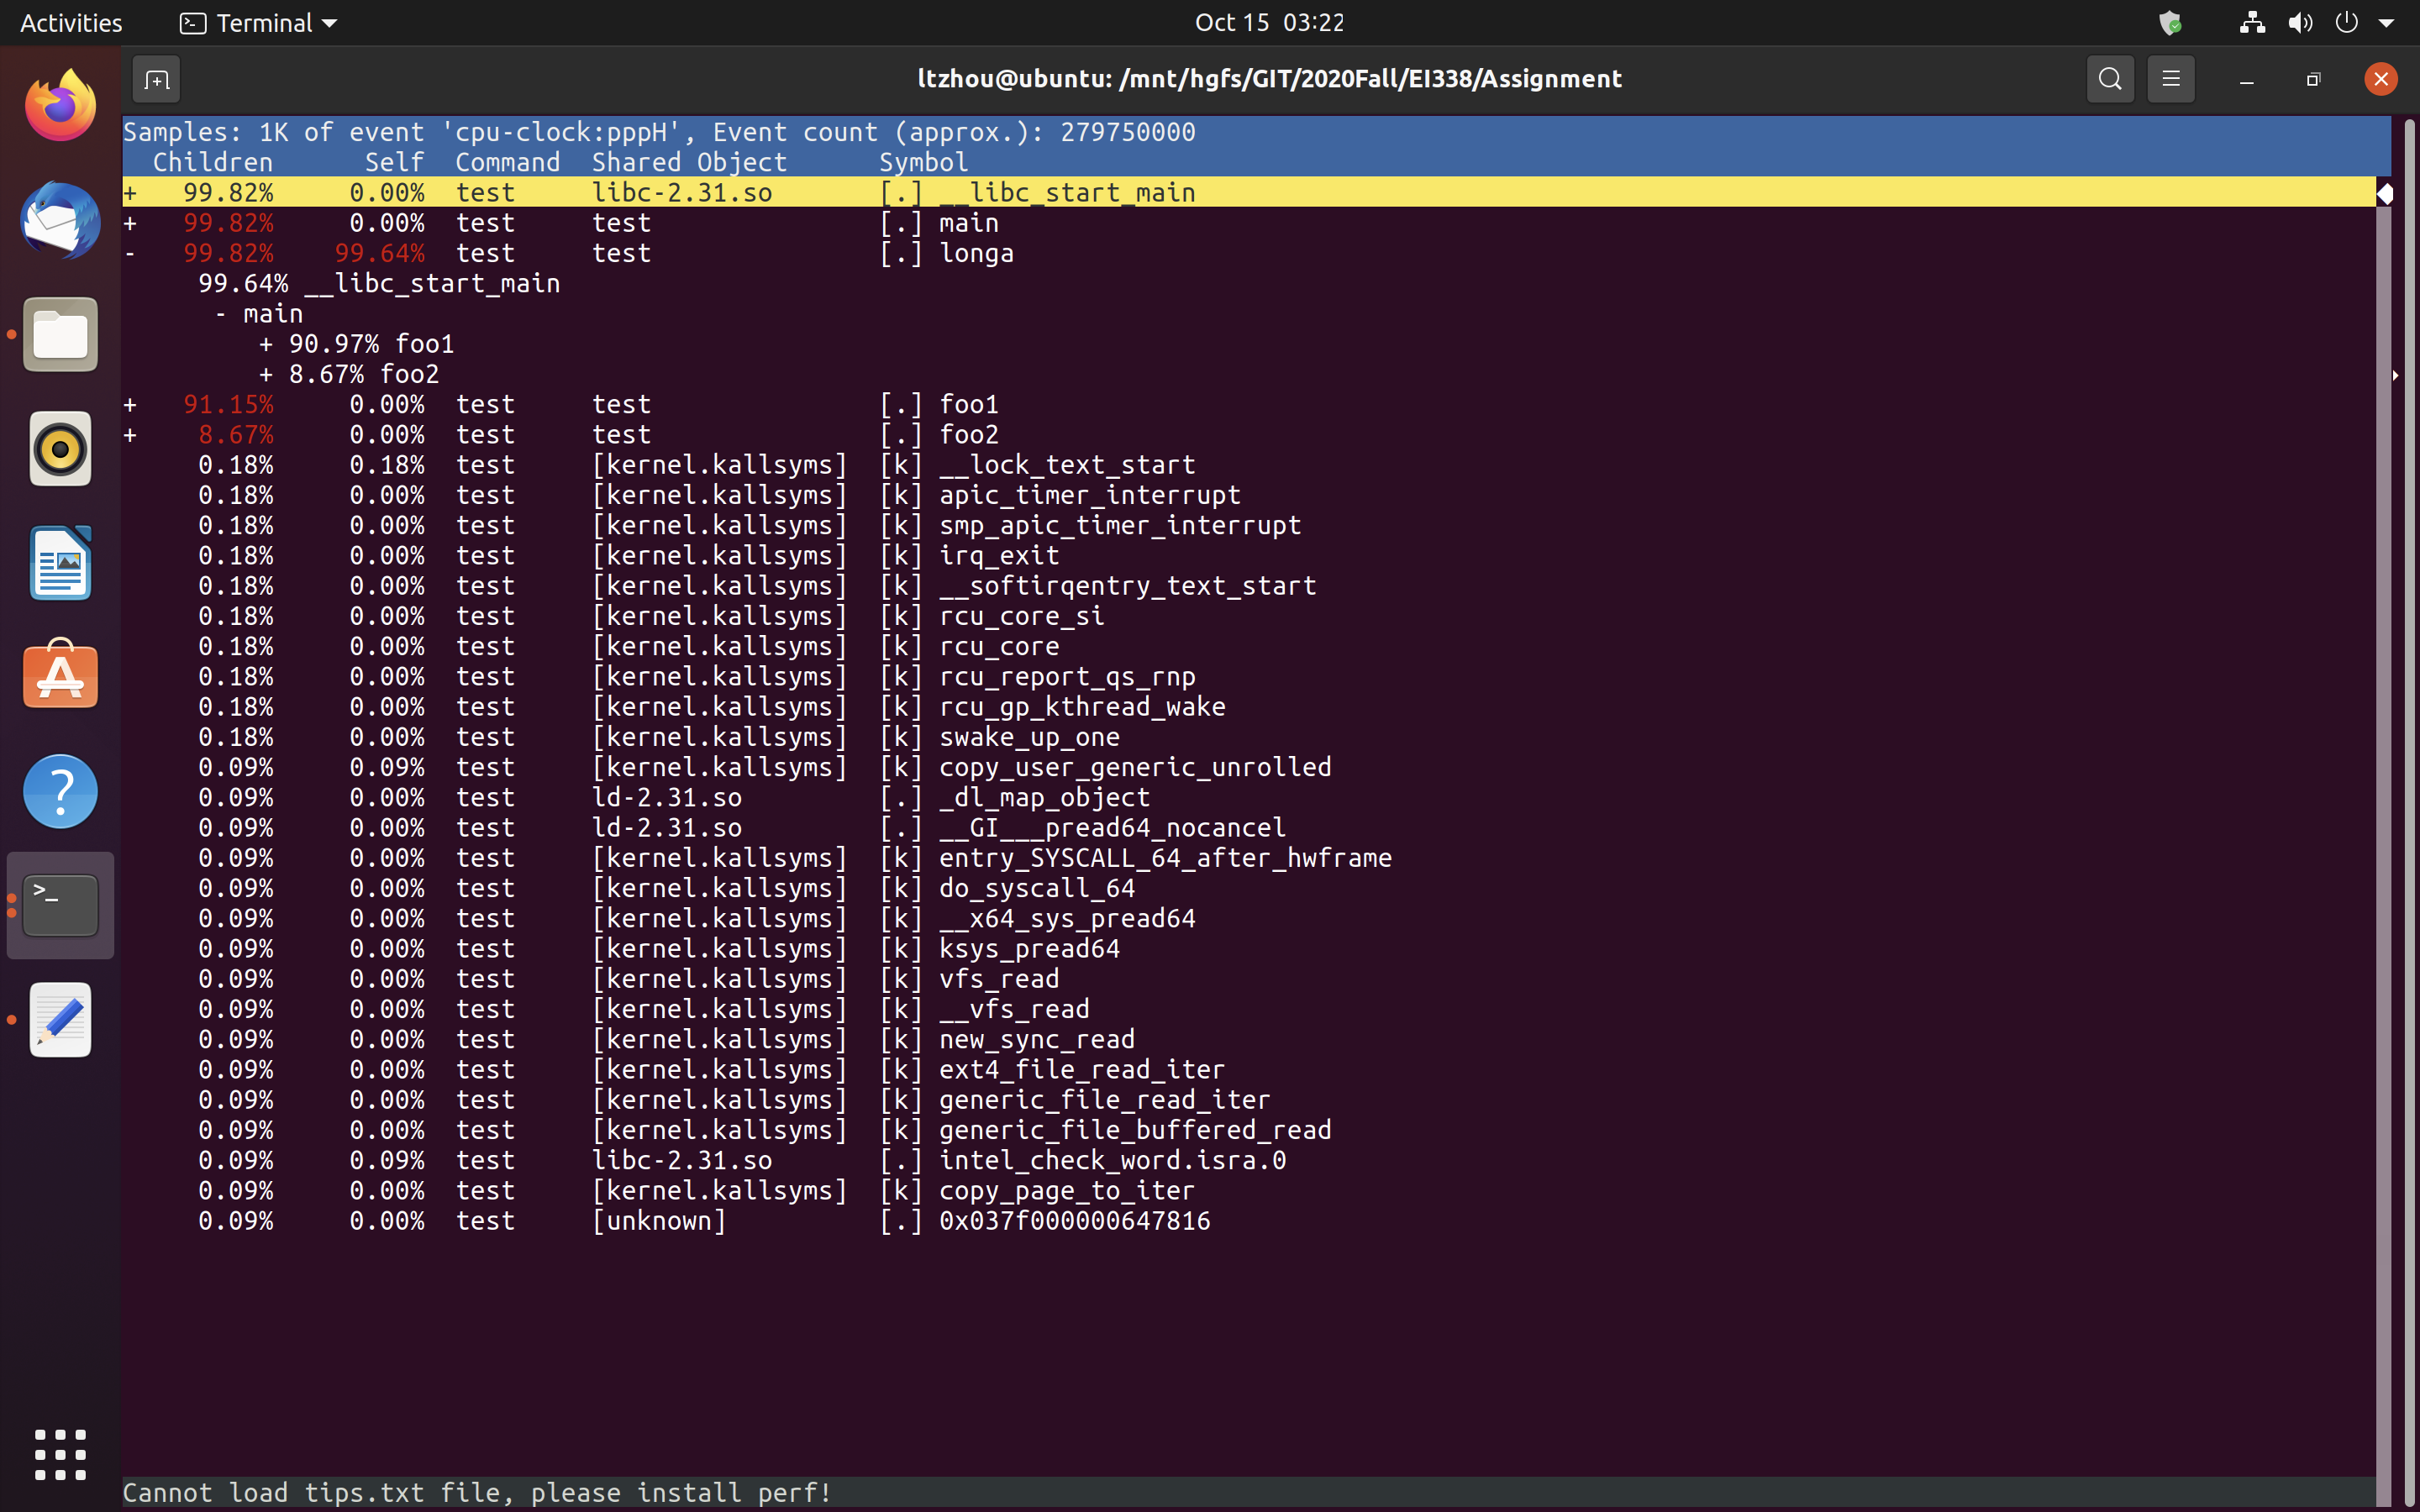
\includegraphics[width=14cm]{perf.png}
    \label{fig:perf}
    \caption{\texttt{perf} analysis result}
  \end{figure}
  \end{solution}
  \label{ex4}
\end{exercise}


